\section{Globales FEM}

Aus zeit gründen nur Modus A. In einem weiteren Schritt die anderen Modi aufbauen und prüfen.
FEM-Analysen zur kontrolle der Handrechnungen.\\
Verformungen\\
Überprüfen ob der Boden geklebt werden kann.\\

Mit dem globalen FEM-Modell sollen folgende Punkte bestimmt werden:
\begin{itemize}
  \item Lagerreaktionen
  \item Kontakt-Reaktion: Chassis - Träger A und B
  \item Kontakt-Reaktion: Chassis - Boden
  \item Biegemoment in Chassis und Dach
  \item Normalkräfte in Chassis und Dach
\end{itemize}

Was wird rausgelesen:\\
Lagerreaktionen: Deichsel, Links, Rechts\\
Träger A und B Reaktionen:\\
Chassis: Max. Biegemoment.\\
Chassis: Max. Normalkräfte\\
Dach: Max. Normalkräfte\\
Boden: Max. Kraftreaktion\\


\subsection{Idealisierung und Modell}
Der Solar Butterfly wird aus Balken und Schalenkörper aufgebaut. Das Chassis, die Träger A und B sowie die Dachträger werden als Balken mit den entsprechenden Querschnitten modeliert. Die Wände, Dächer und der Boden werden das Schalenkörper modelliert, wobei den Schalenkörper jeweils ein Lagenaufbau zugewiesen wird, welcher die Sandwichbauweise nachstellt. In den Abbildungen \ref{FEM Mesh1} ist das komplette Modell des Solar Butterfly zu sehen. In der Abbildung \ref{FEM Mesh3} wurden die Schalenkörper ausgeblendet, sodass nur die Balken sichtbar sind.

\begin{figure}[h]
  \centering
  \begin{minipage}{.5\textwidth}
    \centering
    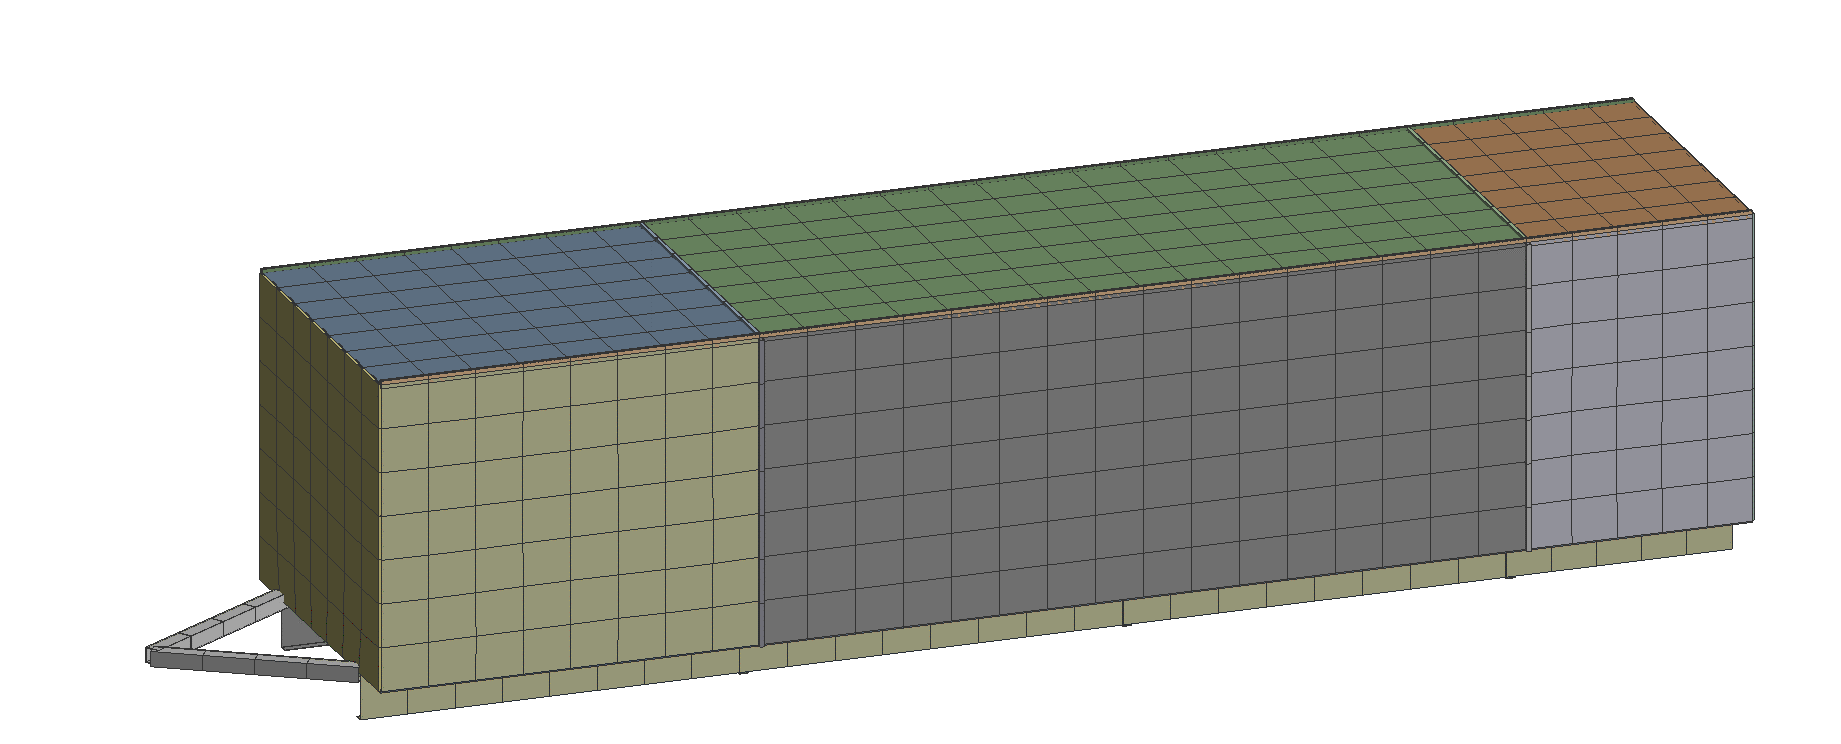
\includegraphics[width=.98\linewidth]{04_figures/FEM Mesh1.png}
    \caption{Darstellung der Balken und Schalenkörper im FEM-Modell}
    \label{FEM Mesh1}
  \end{minipage}%
  \begin{minipage}{.5\textwidth}
    \centering
    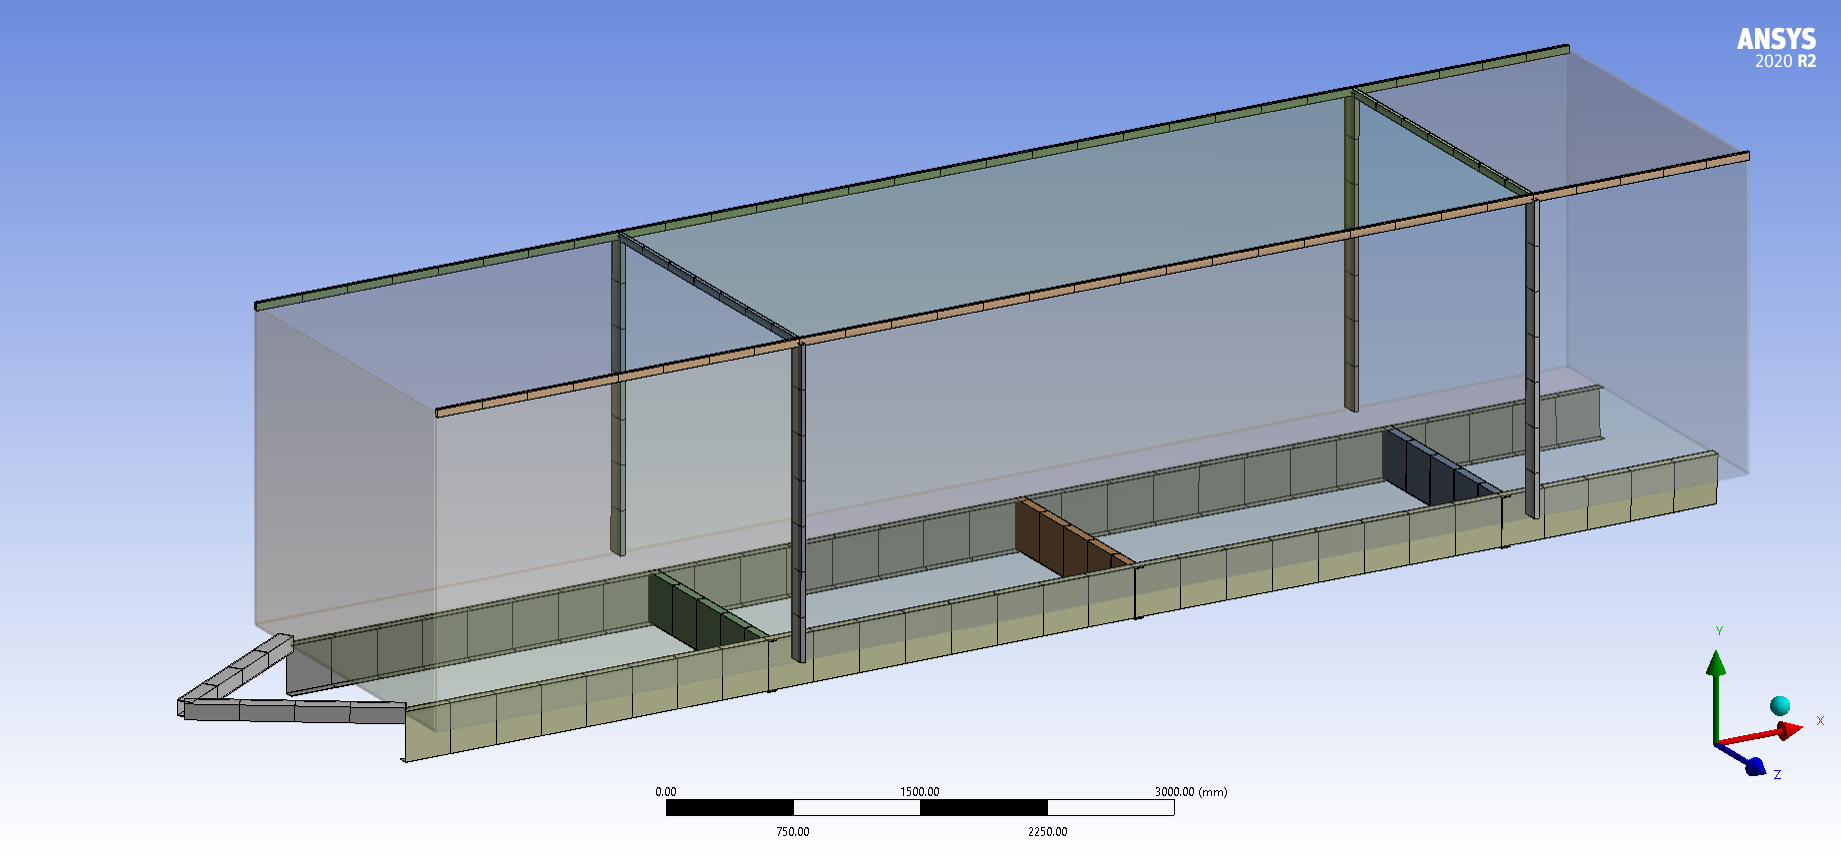
\includegraphics[width=.98\linewidth]{04_figures/FEM Mesh3.png}
    \caption{Darstellung aller Balken im FEM-Modell}
    \label{FEM Mesh3}
  \end{minipage}
\end{figure}

Um die Masse des Solar Butterflys modellieren zu können, werden, zusätzlich zu den Massen der modellierten Bauteilen, Punktmassen (Point-mass) eingeführt. Es werden für die drei Raumelemente Küche, Mittelkörper und Bad je eine Punktmasse definiert, deren Masse und Trägheitsmomente mit der Hilfe der Massenverteilung aus dem Kapitel KAPITEL bestimmt wird. In der Abbildung \ref{img:FEM Punktmasse} ist die Verbindung der Punktmassen mit dem Rest des Modelles dargestellt.\\
Die Deichsel, Längsträger und Querträger des Chassis werden durch das Zusammenführen der deckungsgleichen Koten miteinander verbunden. Auf die selbe Art und Weise werden die Träger A und B, die Längsträger des Daches sowie der Boden, die Wände und die Dächer des Aufbaus miteinander verbunden. Der Aufbau wiederum wird auf zwei Arten mit dem Chassis verbunden. Einerseits werden die Träger A und B über Fixe MPC-Kontakte (alle Freiheitsgrade eingeschränkt) mit dem Chassis verbunden. Weiter wird der Boden über Translatorische MPC Kontakte mit den Längsträgern des Chassis verbunden. Sie stellen die Klebeverbindung des Bodens zum Chassis dar.


!!! Trägheit der Pointmass überprüfen!!!

\begin{figure}[h]
  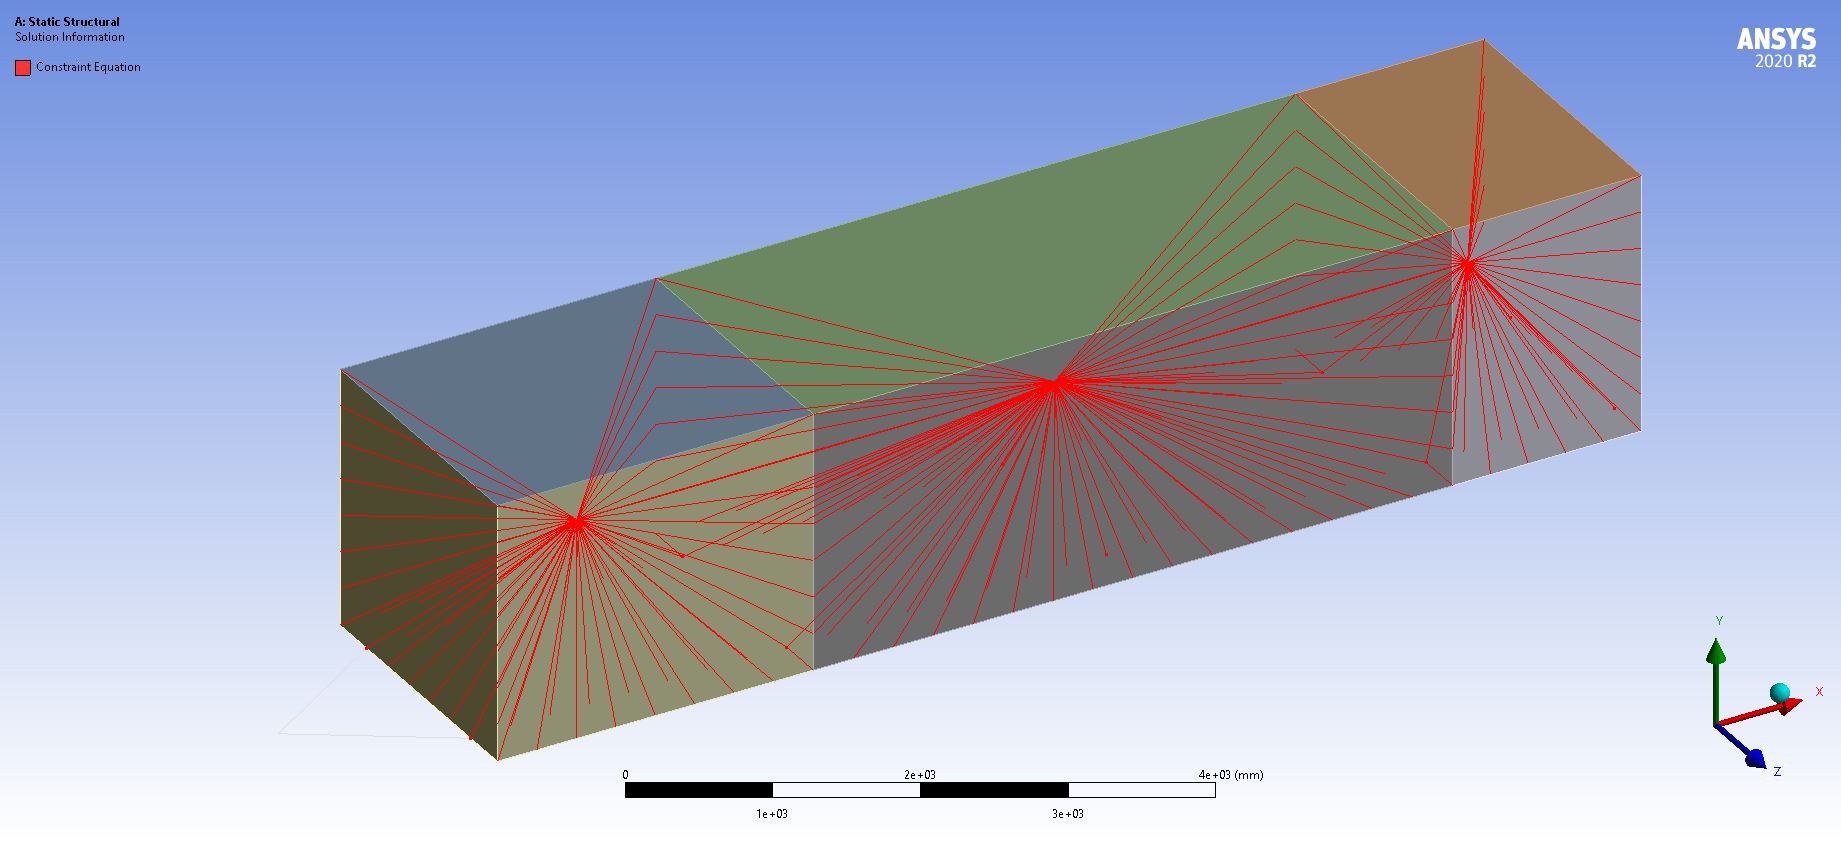
\includegraphics[width=0.5\linewidth]{04_Figures/FEM Punktmasse.png}
  \caption{Darstellung des mittleren Raumelementes}
  \label{img:FEM Punktmasse}
\end{figure}

In allen folgenden FEM-Simulationen ist der Solar Butterfly analog zu den Berechnungen im Kapitel \ref{sub:Longitudinale Beschleunigung} (Lastfall 1.1 \emph{Vertikale Beschleunigung}) gelagert. An der Deichsel sind die rotatorischen Freiheitsgrade freigegeben, die translatorischen jedoch eingeschränkt. An der Achse wird lediglich die Verschiebung in x-Richtung (Fahrtrichtung) zugelassen.





\begin{table}[h!]
\centering
\begin{tabular}{lcccccc}
Grösse	&	Einheit	&	x	&	y	&	z	&	Total	&	Berechnet	\\	\hline
\textbf{Lagerreaktionen}	&		&		&		&		&		&		\\	\thickhline
Deichsel	&		&	0	&	3091	&	0	&	3091	&	-1028	\\
Chassis Links	&	N	&	0	&	33997	&	6476	&	34608	&	37300	\\
Chassis Rechts	&		&	0	&	33997	&	-6476	&	34608	&	37300	\\	\hline	\\
\textbf{Träger A und B}	&		&		&		&		&		&		\\	\thickhline
Normalkräfte A	&	N	&	-604	&	12416	&	-215	&	12433	&		\\
Biegemoment A	&	kNmm	&	-4420	&	-176	&	327	&	4436	&		\\
Normalkräfte B	&	N	&	2381	&	15152	&	679	&	15353	&		\\
Biegemoment B	&	kNmm	&	-5386	&	823	&	-333	&	5459	&		\\	\hline	\\
\textbf{Chassis}	&		&		&		&		&		&		\\	\thickhline
Normalkräfte	&	N	&		&		&		&	-48670	&	-44518	\\
Biegemoment	&	kNmm	&		&		&		&	16360	&		\\	\hline	\\
\textbf{Dach}	&		&		&		&		&		&		\\	\thickhline
Normalkräfte	&	N	&		&		&		&	-10469	&	14840	\\
Biegemoment	&	kNmm	&		&		&		&	314	&		\\	\hline	\\
\textbf{Boden}	&		&		&		&		&		&		\\	\thickhline
Normalkräfte	&	N	&		&		&		&	745	&		\\
Schubkräfte	&	N	&		&		&		&	9286	&		\\	\hline
\end{tabular}
\caption{Vorlagetabelle für Resultate aus FEM}% Add 'table' caption
\label{Resultate Vorlage}
\end{table}







\subsubsection*{Vertikale Beschleunigung}


\subsubsection*{Laterale Beschleunigung}


\subsubsection*{Longitudinale Beschleunigung}


\subsubsection*{Rotatorische Beschleunigung}


\newpage
